\documentclass[a4paper,doc,floatsintext,natbib]{apa6}
% \documentclass{article, a4paper}
\usepackage[font=small]{caption}
\usepackage{lscape}
\usepackage{graphicx}
\usepackage{amsmath}
\usepackage{authblk}
\usepackage[utf8]{inputenc}
\usepackage{nameref}
\usepackage{hyperref}
\usepackage{cleveref}
\usepackage{soul}
\usepackage{todonotes}

% Remember to start reftex-mode

\hypersetup{
  colorlinks=true,
  linkcolor=black,
  citecolor=black,
  urlcolor=black
  }

\setlength{\parskip}{1em}
\def \fref #1{Figure \ref{#1}}     % Reference figures
\def \tref #1{Table \ref{#1}}      % Reference tables
\def \eref #1{Equation \ref{#1}}   % Reference equations
\def \sref #1{Section '\nameref{#1}'}    % Reference sections
\def \supmat {the Supplementary Materials}

\DeclareMathOperator*{\argmin}{argmin}
\DeclareMathOperator*{\argmax}{argmax}

% For revision
\DeclareRobustCommand{\newcontent}[1]{#1}

\title{The effects of context inference on motor learning: savings, de-adaptation and spontaneous recovery}
\shorttitle{Context-inference-dependent motor learning}
\author[1]{Cuevas Rivera, Darío}
\author[1]{Kiebel, Stefan J.}
\affil[1]{Chair of Neuroimaging, Faculty of Psychology. Technische Universität Dresden, 01062 Dresden, Germany.}
\affiliation{~}

\begin{document}

\maketitle

\abstract{Abstract}
Very interesting abstract. Much wow.

\section{Introduction}
It has been long known that humans are capable of learning multiple novel motor tasks at the same time, even when these tasks oppose each other \citep[e.g.][]{Gandolfo_Motor_1996,Shadmehr_Functional_1997}, although interference can occur between tasks \citep[e.g.][]{Brashers-Krug_Consolidation_1996,Sing_Reduction_2010}.

In order to study motor adaptation, motor error is defined as the deviation between the observed movements of a participant and a baseline movement. For example, in experiments with a mechanical arm \citep[e.g.][]{Gandolfo_Motor_1996}, a correlation coefficient is defined between the movements when the mechanical arm exerts a force and the movements when it does not; the higher the correlation coefficient, the lower the error. Other examples include measuring the force profile in error-clamp trials \citep{Smith_Interacting_2006}, endpoint errors in visuomotor rotations \citep{Kim_Neural_2015} and saccade adaptation \citep{Catz_Cerebellardependent_2008}.

By introducing blocks of trials in which a manipulation is present (e.g. the mechanical arm exerts a force), experimenters are able to observe the dynamics of adaptation through the lens of motor error. A number of phenomena have been observed that persist across participants and across many different motor adaptation experiments: savings, quick de-adaptation, anterograde interference and spontaneous recovery.

In order to explain these phenomena, a number of computational models have been introduced. The least complex of these models are linear learners \citep[e.g.][]{Smith_Interacting_2006,Forano_Timescales_2020,Scheidt_Learning_2001}, in which a single one-dimensional variable is used to describe the adaptation of motor commands given the observed motor errors. By having multiple time scales, each with a learning rate and a forgetting rate, these models have been fitted to experimental data, explaining these distinct experimental phenomena.

Bayesian accounts of motor adaptation have also been previously presented, providing an alternative explanation for savings and quick de-adaptation in the form of switching between internal models of adaptation via predictions generated by these internal models \citep{Kording_Bayesian_2004,Oh_Minimizing_2019}. These models replace the idea of explicit multiple time scales with an estimation of their own uncertainty: as the model practices the same task, the uncertainty on its estimate of the underlying modification is reduced, which lowers variability in responses, as well as increases the stability of the estimate.

While these general models of adaptation explain the most common phenomena observed in experiments, a number of known phenomena remain outside of their scope. For example, it is known that adaptation rate is reduced in situations where the environment is unstable and unpredictable \citep{Herzfeld_memory_2014}, or situations in which errors are small \citep{Marko_Sensitivity_2012} and slowly introduced \citep{Huang_Persistence_2009}. Learning new adaptations has been found to depend on the history of adaptations learned \citep{Vaswani_Decay_2013}, as well as the way in which those adaptations were presented [CITATION NEEDED]. 

In this work, we present a computational model for motor adaptation inspired by models such as MOSAIC \citep{Wolpert_Multiple_1998} and Bayesian switching models \citep{Kording_Bayesian_2004,Oh_Minimizing_2019}. We expand on these models by expanding the concept of context and introducing an explicit mechanism for inferring the context based on Bayesian inference. In our model, the context encompasses all the information relevant to making decisions, both environmental and internal to the agent making these decisions. To infer the current context, our model integrates several sources of information, including the predictions made by its internal forward models, an estimate of the reliability of these predictions, direct sensory information (such as visual contextual cues), proprioceptive information, and feedback provided by the environment. Having inferred the context, the model can choose the best-fitting internal model with which to make decisions.

We show that the dynamics of context inference provide a unifying explanation for all the experimental phenomena outlined above, providing a single account for motor adaptation under changing contexts, while relying on known mechanisms for adaptation.

\section{Results}
In this work, we present a motor adaptation model in which the agent (e.g. a human learning a motor task) updates an existing model of the environment based on error signals produced by the need of adaptation. Several models exist for error-based motor adaptation, but we expand on the existing models by adding an explicit component of context inference which guides the selection of the adequate internal model, its updating and the sampling of actions.

We used our model to explain several experimental phenomena found in previous studies. We simulated representative experiments from these studies to show how our model explains their findings using the dynamics of context inference. In what follows, we will present these simulations alongside the experimental data from the representative studies and discuss how context inference explains the data.

Before presenting our simulations, we will briefly explain the fundamentals of the model we present. We leave the mathematical details of the implementation to the Methods section.

\subsection{The model}
The model we present has three main components: (1) context-inference, (2) motor adaptation and (3) action selection. Each of these components informs the ones that follow: motor adaptation is informed by context inference, and action selection is informed directly by both motor adaptation and by context inference.

We now briefly describe the three components of the model separately. For clarity, we start with the second component (i.e. motor adaptation), in order to introduce the terminology that we use throughout this work.

\subsubsection{Motor adaptation}
Motor adaptation refers to the ability of humans and other animals to adapt their motor commands based on performance errors. For example, we can learn to perform a reaching movement in front of us underwater, where the relatively high viscosity of water means that the motor commands we have learned all our lives no longer produce the desired effect.

It is widely accepted that in order to adapt motor commands to a novel environment, we create and update internal forward models of the outcomes of control signals \citep{Wolpert_Multiple_1998}. We chose to make use of an exact Bayesian learner. As we discuss below, a Bayesian learner has the advantage of not only fitting experimental data on motor adaptation, but also eliminates the need for explicit multiple time scales of learning. We show that this adaptation mechanism can deal with adaptation after any number of trials, ranging from a handful of trials in an experiment to the level of expertise a professional dancer has accrued through years of practicing the same movements.

To describe this component of the model, we make use of the example of reaching movements. Throughout our lives, we have learned the equivalence between a motor command and its outcomes in the form of a forward model. We can write this forward model as follows:
\begin{equation}
p(\vartheta | s, c) = f(s, c; \phi) \label{eqn:forward-model}
\end{equation}
where $\vartheta$ are the outcomes of an action (in the example, direction and velocity of the hand during the reaching movement), $s$ is the current state (e.g. the current position of the hand), $c$ is a motor command and $\phi$ are the parameters of the forward model $f(\cdot)$. Throughout our lives, the parameters $\phi$ have been fine tuned to produce an accurate forward model $f$ to guide our movements and it is these parameters which are updated during motor adaptation.

When an observed outcome does not match the predictions produced by $f$, the prediction error is used to update the parameters $\phi$ of the forward model. To describe this adaptation process, our model makes uses of Bayesian inference, such that:
\begin{equation}
q(\phi | \vartheta, s, c) \propto p(\vartheta | s, c, \phi)p(\phi)
\end{equation}
where $q(\phi | ...)$ represents the new estimate of $\phi$ after having observed the outcome $\vartheta$ of the previous motor command $c$. The likelihood $p(\vartheta | s, c, \phi)$ is the \textit{a priori} probability of observing the outcome $\vartheta$ as predicted by the forward model $f$, and $p(\phi)$ is the previous estimate of $\phi$.

\subsection{Context inference}
In our model, the idea of context is quite general. The context comprises the relevant elements of the environment (e.g. the strength and direction of the wind when walking) and of the task at hand (immediate and long-term goals, reward structure, etc). Previous models \cite[e.g.][]{Wolpert_Multiple_1998,Imamizu_Neural_2008,Oh_Minimizing_2019} have focused on the elements of the context which are directly related to the internal models: given a past action, the different internal models (e.g. two forward models $f_B$ and $f_H$) make different predictions for the outcome of that action; the model that best predicts that action is deemed to be the ``correct'' model, i.e. the model that best represents the context.

In this work, we expand on this idea of switching internal models by creating context inference that integrates several sources of information, including sensory cues, outcome prediction errors and reward prediction errors.

Identifying any possible context with a categorical variable $\zeta$, the identification of a context is done by our model through Bayesian inference:
\begin{equation}
q(\zeta | \vartheta_t, \vartheta_{t-1}, c_{t-1}) \propto p(\vartheta_t | \vartheta_{t-1}, c_{t-1})p(\zeta)
\end{equation}
where the prior distribution over contexts $p(\zeta)$ includes information from two sources: (1) an expectation of continuity, encoding the expectation that the context does not change from trial to trial, and (2) an overall estimation of observing any one context, if the context did change. Below, we discuss how these two components effect different experimentally observed phenomena.

In the previous section, we used the variable $\vartheta$ to refer to the outcomes of actions. In this section, we expand the definition of an observation $\vartheta$ to include any information given to the decision-making agent by the environment. This includes, as before, the outcomes of actions (e.g. the new position of the hand), but also any other sensory information that might be indirectly related to actions, or even completely independent from them. For this section, the most important component of $\vartheta$ is contextual sensory information, i.e. information that might directly help infer the identity of the current context.

In experimental settings, the contextual sensory information can take the form of a visual cue \cite[e.g.][]{Lee_Dual_2009,Kim_Neural_2015}, the place where the task must be carried out \cite[e.g.][]{Forano_Timescales_2020,Shadmehr_Adaptive_1994} or even the start of a new block of trials \cite{Ethier_Spontaneous_2008}. All these sources of information, alongside the outcomes of previous actions and the priors $p(\vartheta)$ form part of $p(\vartheta_t | \vartheta_{t-1}, c_{t-1})$ and are integrated together to identify a context.

By making use of NormalGamma priors on context, the model performs exact Bayesian inference at every trial. The exact update equations can be found in the Methods section.

\subsection{Action selection}
Action selection is affected by the current context via the context-dependent forward model that is used. In our model, action selection is made by building a distribution over available actions which is a weighted sum of the distributions given by the existing forward models, where the weights are obtained by the context inference component of the model. In other words, a distribution is created as follows:
\begin{equation}
p(c_t) \propto \displaystyle\sum_{\zeta \in \Phi}q(\zeta | \vartheta_t, \vartheta_{t-1}, c_{t-1}) p(c_t | \zeta)
\end{equation}
where $p(c_t | \zeta)$ corresponds to \eref{eqn:forward-model}. From this distribution, the current action (motor command $c_t$) can be sampled and carried out.

\section{Experimental results}
In this section, we go through a number of experimentally-observed phenomena and show that context inference, as done in our model, provides a parsimonious explanation for all of them.

For clarity, we introduce some terminology before discussing these phenomena. As an example, we will use a typical motor adaptation task in which participants have to make forward-backward reaching movements while holding the handle of a mechanical arm that exerts a force. Depending on the trial, the arm might exert a curl force in a clockwise or counter-clockwise direction, or no force at all. Let us define the baseline context O as that in which the mechanical arm exerts no force. Context A can be defined as that in which the arm exerts the clockwise curl force and context B counter-clockwise. Additionally, abusing notation, it can be said that $B = (-A)$, as the forces point in opposite directions. We can also talk of contexts such as A and A/2, which means that both have the same direction of the adaptation (e.g. clockwise), but the second one has half the magnitude. Finally, error-clamp trials, in which the mechanical arm forces the participant to make straight-line movements, are represented with the letter E.

With this terminology, a typical experiment \cite[e.g.][]{Ethier_Spontaneous_2008} would have a block structure of O-A-B-E, or O-A-(-A)-E, which means that the participant goes through a block of trials with no external force applied (O), a number of trials with a clockwise curl force (A), a block with counter-clockwise forces (B), and finally a block with error-clamp trials (E).

\subsection{Savings}
Savings refers to the ability of humans and other animals to remember a previously-learned adaptation and apply it without having to re-learn it. Savings is almost universally observed in human participants \cite{Brashers-Krug_Consolidation_1996,Shadmehr_Functional_1997,Medina_Mechanism_2001,Smith_Interacting_2006,Zarahn_Explaining_2008}. In an O-A-O-A experiment, for example, savings would be seen in the second A block in the form of a much higher adaptation rate higher than that observed during the first A block.

In this section, we discuss savings, and the related phenomenon of deadaptation, in terms of the switching between forward models. This has been modeled before \citep[e.g.][]{Wolpert_Multiple_1998,Oh_Minimizing_2019}, but we show that expanding switching into context inference explains facets of savings that these previous models do not.

To show this, we categorized experiments by looking at the amount of contextual information made available to participants. In some experiments \citep[e.g.][]{Kim_Neural_2015,Lee_Dual_2009}, the context is clearly revealed to the participant. We call these cued-context experiments. In other experiments, partial information is available to participants \citep[e.g.][]{Davidson_Scaling_2004,Zarahn_Explaining_2008} in the form of large prediction errors, partial contextual information or reward prediction errors; we refer to these as partially-cued experiments.

To our knowledge, there are no experiments in which no contextual information is available. However, many experiments \citep[e.g.][]{Huang_Persistence_2009,Brennan_Decay_2015,Smith_Interacting_2006} contain blocks of error-clamp trials in which participants have no way of identifying the current context. These blocks could be considered uncued, however, as we discuss in the following sections, contextual information is still available to participants.

In this section, we focus on cued and partially-cued experiments and leave error-clamp trials to the following sections.

Note that, because context inference integrates information from many sources, many experiments in which no intentional, overt contextual cues are available indeed contain contextual information that the participant can use. For example, in curl-force-field experiments with mechanical arms, the force feedback provided by the mechanical arm always gives participants a sense for the current context, although error-clamp trials are difficult to distinguish from adaptation trials based on force feedback alone. In fact, the mere act of holding the handle informs participants that something is different from baseline. Proprioceptive signals can also provide contextual information \cite{Dizio_Motor_1995,Shadmehr_Adaptive_1994}. The sudden appearance of motor errors can itself be a cue for contextual change, as long as the motor error is perceivably higher than normal trial-by-trial variation in performance, and even an unusually long pause between two trials could indicate to participants that a new block with a potentially different context could have started \cite[e.g.][]{Ethier_Spontaneous_2008}.

To show how adaptation changes depending on the amount of contextual information, we selected three representative experiments from two studies which differ in the amount of contextual information. \cite{Kim_Neural_2015} performed a visuomotor rotation experiment with three contexts with different rotation: no rotation, 40 degrees and -40 degrees. Participants performed shooting movements in blocks of trials with the same rotation. Importantly, the identity of the current context was displayed as a visual cue (colored light), making this a cued-context experiment. Consistent with our model, the authors found that switching was immediate and accurate. In \fref{fig:oh-2019}A we show the results of simulations with our model using the parameters of the task, as well as the experimental results from \cite{Kim_Neural_2015}. The correspondence between simulations and experimental results is quite evident, both in the immediacy of the switches as well as in the fact that learning continues from the state it was when the context was last observed.

\begin{figure}
\centering
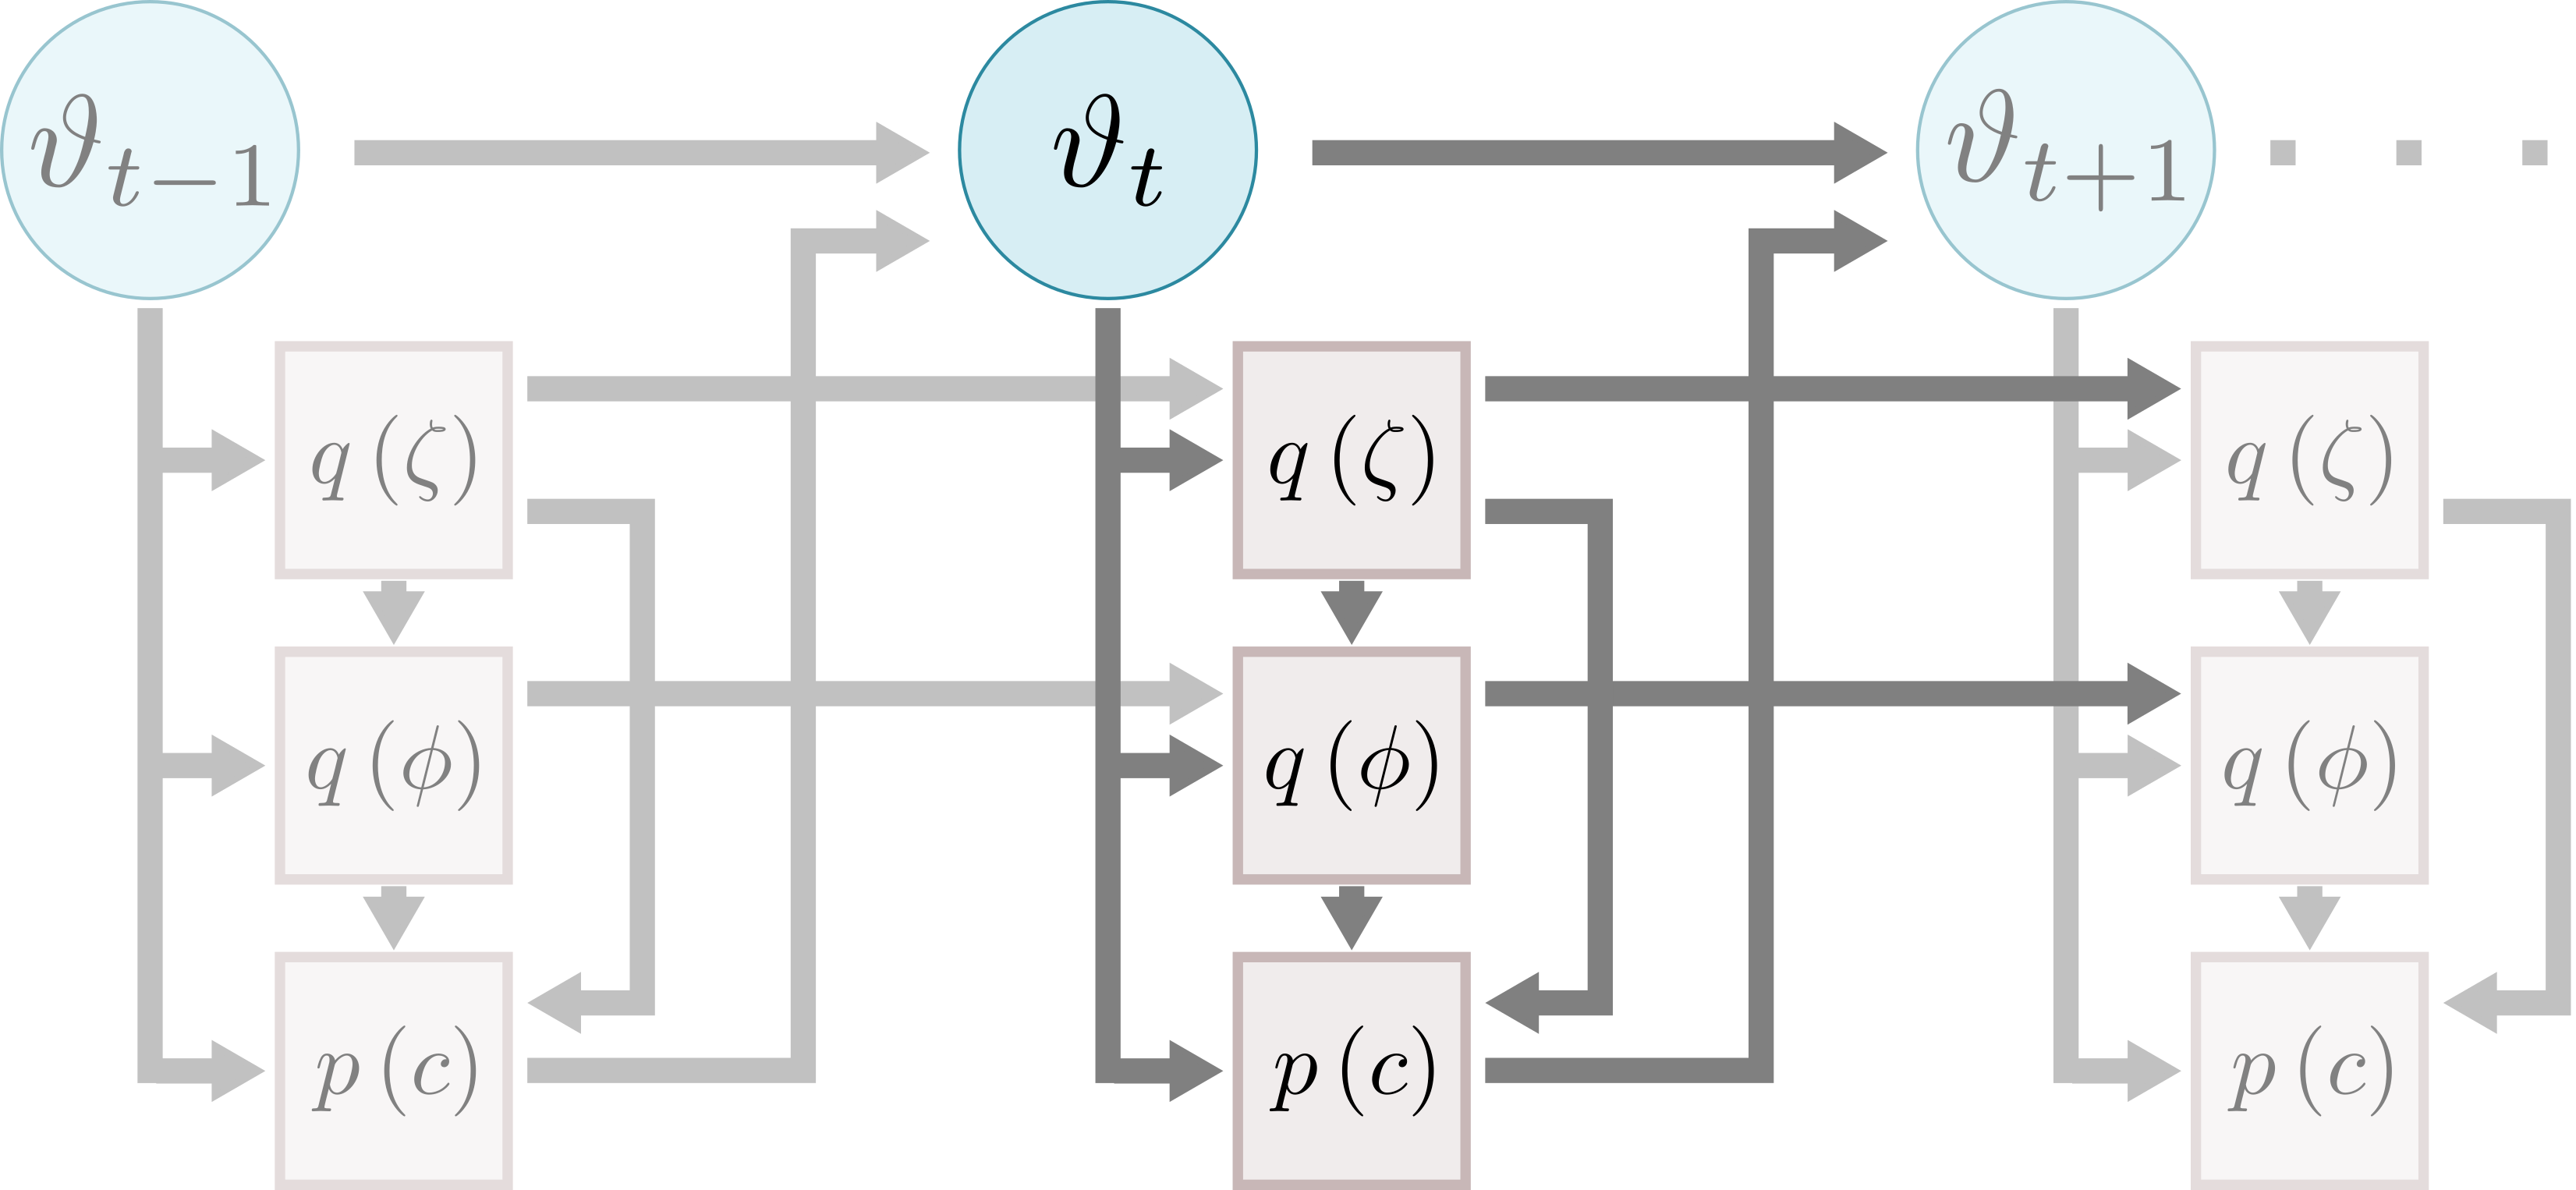
\includegraphics{./figures/figure_1.png}
\caption{Savings and de-adaptation. Data from our simulations (left column) compared to data from \cite{Kim_Neural_2015} and \cite{Oh_Minimizing_2019} (right column). In all panels, the blue line represents the adaptation displayed by the agent as a function of trial number. The black lines represent the optimal adaptation, i.e. the size of the visuomotor rotation during the task. (A) Experiment by \cite{Kim_Neural_2015} with two rotations (-40 and 40 degrees), in addition to baseline. The switches between contexts were visually cued and therefore switches are immediate, as can be seen in both simulations (left) and the experimental data from \cite{Kim_Neural_2015} (right). (B) An experiment in which the agent must adapt to a 20 degree visuomotor rotation during shooting movements. It can be seen in both the simulations (left) and experimental data from \cite{Oh_Minimizing_2019} (right) that after context switches (e.g. at trial 120), the agent returns to the adaptation of the previous block, with one or two trials of delay. (C) Same experiment as (B) but  with a 10 degree adaptation. In this case, savings are much slower.} \label{fig:oh-2019}
\end{figure}

\cite{Oh_Minimizing_2019} performed a similar experiment in which contexts were not visually cued. In addition, the authors performed two experiments that differed in the size of the adaptation: in the first experiment, the angle of rotation was 20 degrees, while in the second experiment it was only 10. The results of their experiments can be seen in \fref{fig:oh-2019}B and \ref{fig:oh-2019}C, respectively, alongside simulations with our model. \cite{Oh_Minimizing_2019} immediate switching in the first experiment, while switching was much slower in the second experiment. As can be seen on the left panels in \fref{fig:oh-2019}B and \ref{fig:oh-2019}C, the same model parametrization produces fast, accurate switches when the adaptation is large, and slow, noisy switches when it is low. This difference is explained by our model in terms of the size of the adaptation: the smaller the adaptation is, the more difficult it is for the agent to notice when the context has changed. Because of this, the model requires more evidence (i.e. more trials) to infer a switch in contexts.

Note that the data from \cite{Oh_Minimizing_2019} and \cite{Kim_Neural_2015} include both savings (O-A transitions) and de-adaptation (A-O transitions), both of which display the same characteristics and are explained by the same mechanism in our model.


\section{The effects on the rate of adaptation}
In our model, adaptation is gated by the uncertainty on the current context. More specifically, a prediction error observed at trial $t$ will effect motor adaptation with a magnitude proportional to the size of the error, where the proportionality constant is related to the uncertainty over the context in which the error was observed: the higher the uncertainty, the lower the size of the adaptation.

The most direct evidence for the effects of context inference on the rate of adaptation come from the experiments by \cite{Herzfeld_memory_2014}. The authors showed that the volatility of the environment, expressed in terms of unpredictable, stochastic transitions between A and -A (and vice versa) change the speed at which adaptation occurs.

\cite{Herzfeld_memory_2014} used an experimental paradigm in which the force that a mechanical arm exerts on the participant's hand can change from trial to trial between O, A and -A. They divided participants into three groups for which the context transition from one trial to the next was very uncommon, somewhat common and almost every trial. Importantly, these transitions were uncued, and the participant could only infer that a transition had occurred after a motor error was observed.

\cite{Herzfeld_memory_2014} found that the volatility of the environment affects learning. The more volatile the environment, the less participants adapt their motor responses after observing an error. In \fref{fig:herzfeld-2014}, we show results obtained with our model in a paradigm matching that of \cite{Herzfeld_memory_2014}. We simulated the conditions of low volatility and maximum uncertainty ($z = 0.9$ and $z = 0.5$ in \cite{Herzfeld_memory_2014}) for thirty trials, repeating the experiment 300 times with random sequences of A and -A each time, following the transition probabilities from the experiment. In \fref{fig:herzfeld-2014}A we show the adaptation as a function of trial number, averaged across all 300 runs. It can be seen that the agent learns more slowly on the more volatile environment ($z = 0.5$) than on the less volatile one, matching the results from \cite{Herzfeld_memory_2014}. Additionally, \fref{fig:herzfeld-2014}B shows the sensitivity to errors, here defined as $\text{adaptation} / \text{error}$; the more volatile environment creates a lower sensitivity to errors than the predictable environment, a difference that is consistent across all trials.

\begin{figure}
\centering
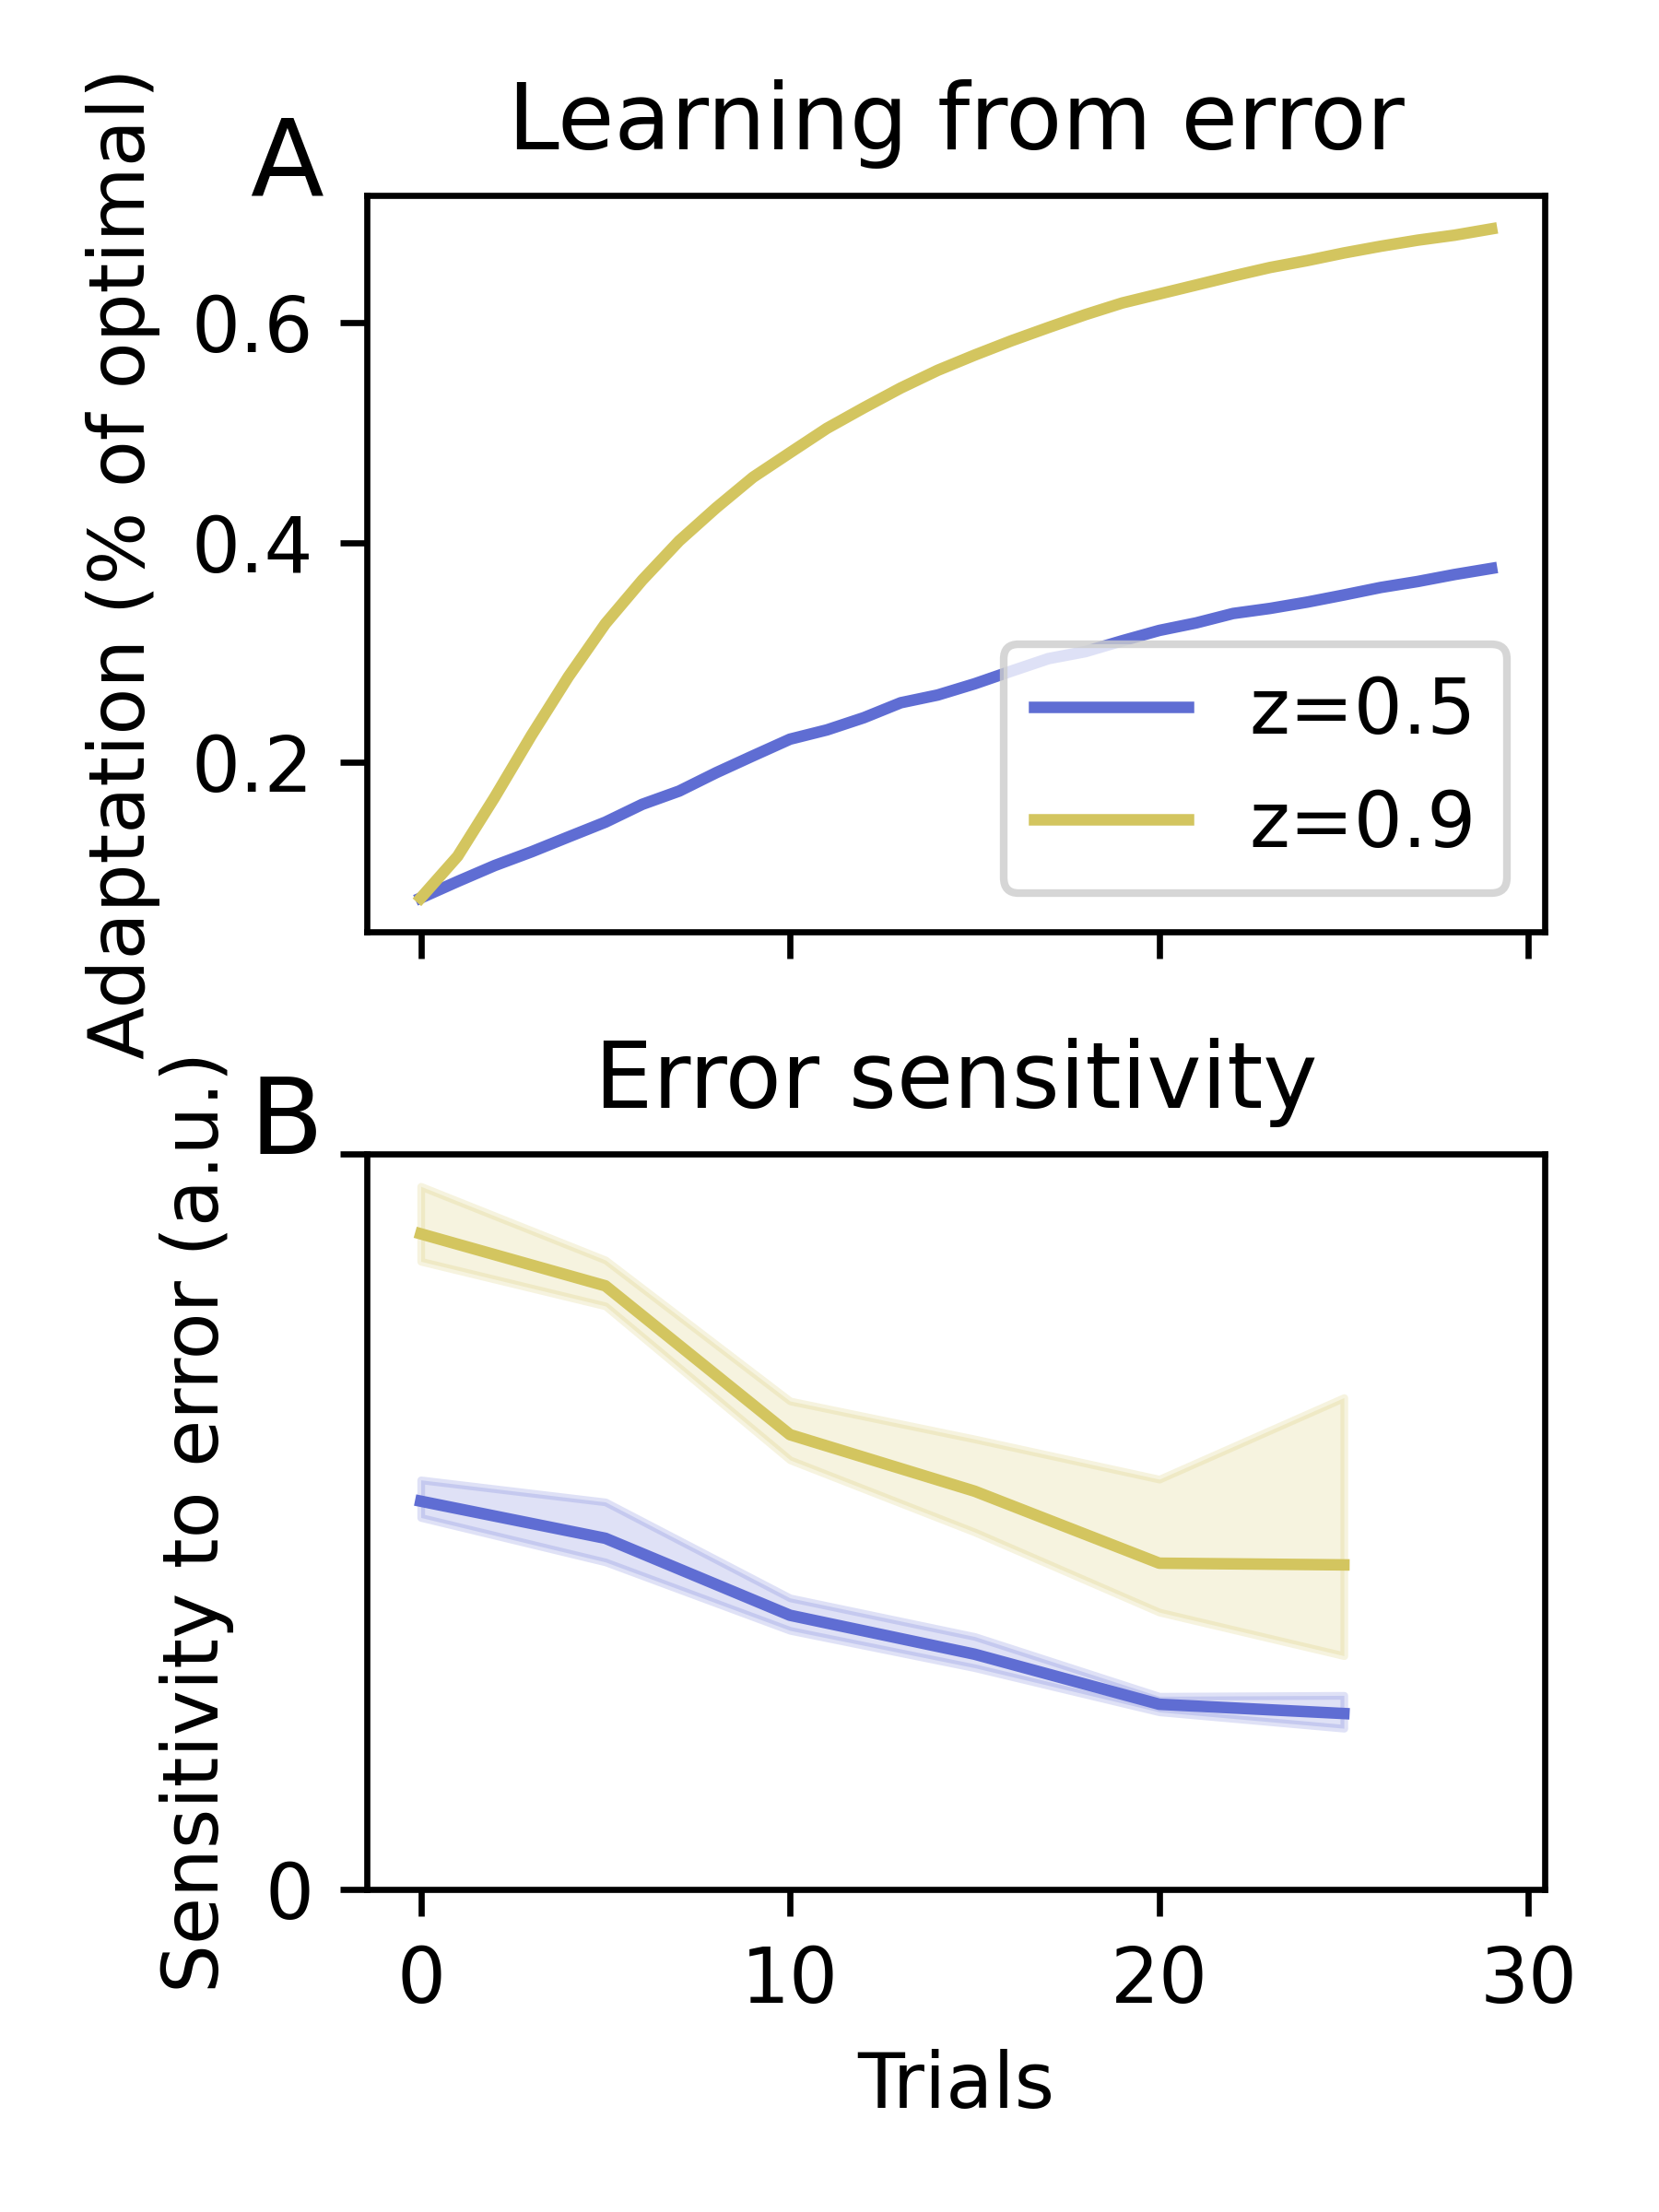
\includegraphics{./figures/figure_2.png}
\caption{Learning under unstable and unpredictable contexts. 30 trials were simulated in the task defined by \cite{Herzfeld_memory_2014}, repeated 300 times for better statistics. Two conditions were used, following the naming convention from \cite{Herzfeld_memory_2014}: $z=0.5$ is an unpredictable condition, where the context has a 0.5 probability of switching from trial to trial. $z=0.9$ is a stable condition, where the context has a 0.9 probability of staying the same from trial to trial. (A) Adaptation as a function of trial number, averaged across all runs. (B) Error sensitivity, binned into bins of 5 trials, averaged across all runs. The error is in arbitrary units, causing sensitivity to error (y axis) to also be in arbitrary units. Shaded areas are SEM.}
\label{fig:herzfeld-2014}
\end{figure}

To account for volatility, our model includes a term in context inference which assumes a transition from the previous context to all other possible contexts (see Methods). Effectively, this transition term gives the model uncertainty on the current context, regardless of observations. The higher the volatility, the higher the uncertainty. This higher uncertainty is what lowers the observed learning rate across all trials.

\section{Action selection}
As with learning, our model selects actions (motor commands) based on context inference. If the identity of the current context is known, the forward model for this context is used to select the current action. However, if uncertainty over the context exists, the selected action is influenced by all the possible contexts, with a weight directly related to how likely each one of those contexts is.

Experimental evidence supporting this view can be found in experiments with context switching. For example, \cite{Davidson_Scaling_2004} reported an experiment in which participants had to switch from 3A to A in one group, with a block sequence A-3A-A-3A, and from -A to A in another group, with a block sequence A-(-A)-A-(-A). After A and 3A (or -A in the other group) had been learned in the first two blocks, the authors found that the switch from 3A to A was faster than that from -A to A. The authors interpreted this as evidence that switching between adaptations happens more quickly if it is in the same direction as the current adaptation (e.g. both counter-clockwise), and more slowly if they are in the opposite direction (e.g. clockwise to counter-clockwise).

Our model offers a different explanation for the observed results: the assymetry is due to the existance of the baseline context. As discussed above, action selection in our model is done via a weighted avarage:
\begin{equation}
p(a_t | s_t) \propto \displaystyle \sum_{m \in M} p(m | s_t, s_{t-1}, a_{t-1}) p(a_t | m)
\end{equation}
In experiments without cued contexts, the baseline model $m_O$ has a non-zero probability $p(m | s_t ...)$. When a new block of trials starts (e.g. in the transition from 3A to A), a switch is inferred by the model (given feedback after the first trial) and $m_O$ becomes more likely (given that $m_{3A}$ has been ruled out. Therefore, in these first trials, action selection has a component guided by the baseline model, in which no extra compensatory force is applied, essentially ``pulling'' adaptation towards zero (no compensatory force). In the first group, this initial pull towards zero accelerates the transition towards A because $3A > A > 0$, but on the second group, it slows down the switch because $A > 0 > -A$.

We simulated data with our model fitting the experimental structure in \cite{Davidson_Scaling_2004}. We show the results in \fref{fig:davidson-2004}, alongside the experimental results from \cite{Davidson_Scaling_2004}. It can be seen that the agent exposed to the -8 context shifts back to 4 more slowly than the one exposed to +8, qualitatively reproducing the data from \cite{Davidson_Scaling_2004}, shown in \fref{fig:davidson-2004}B.

\begin{figure}
\centering
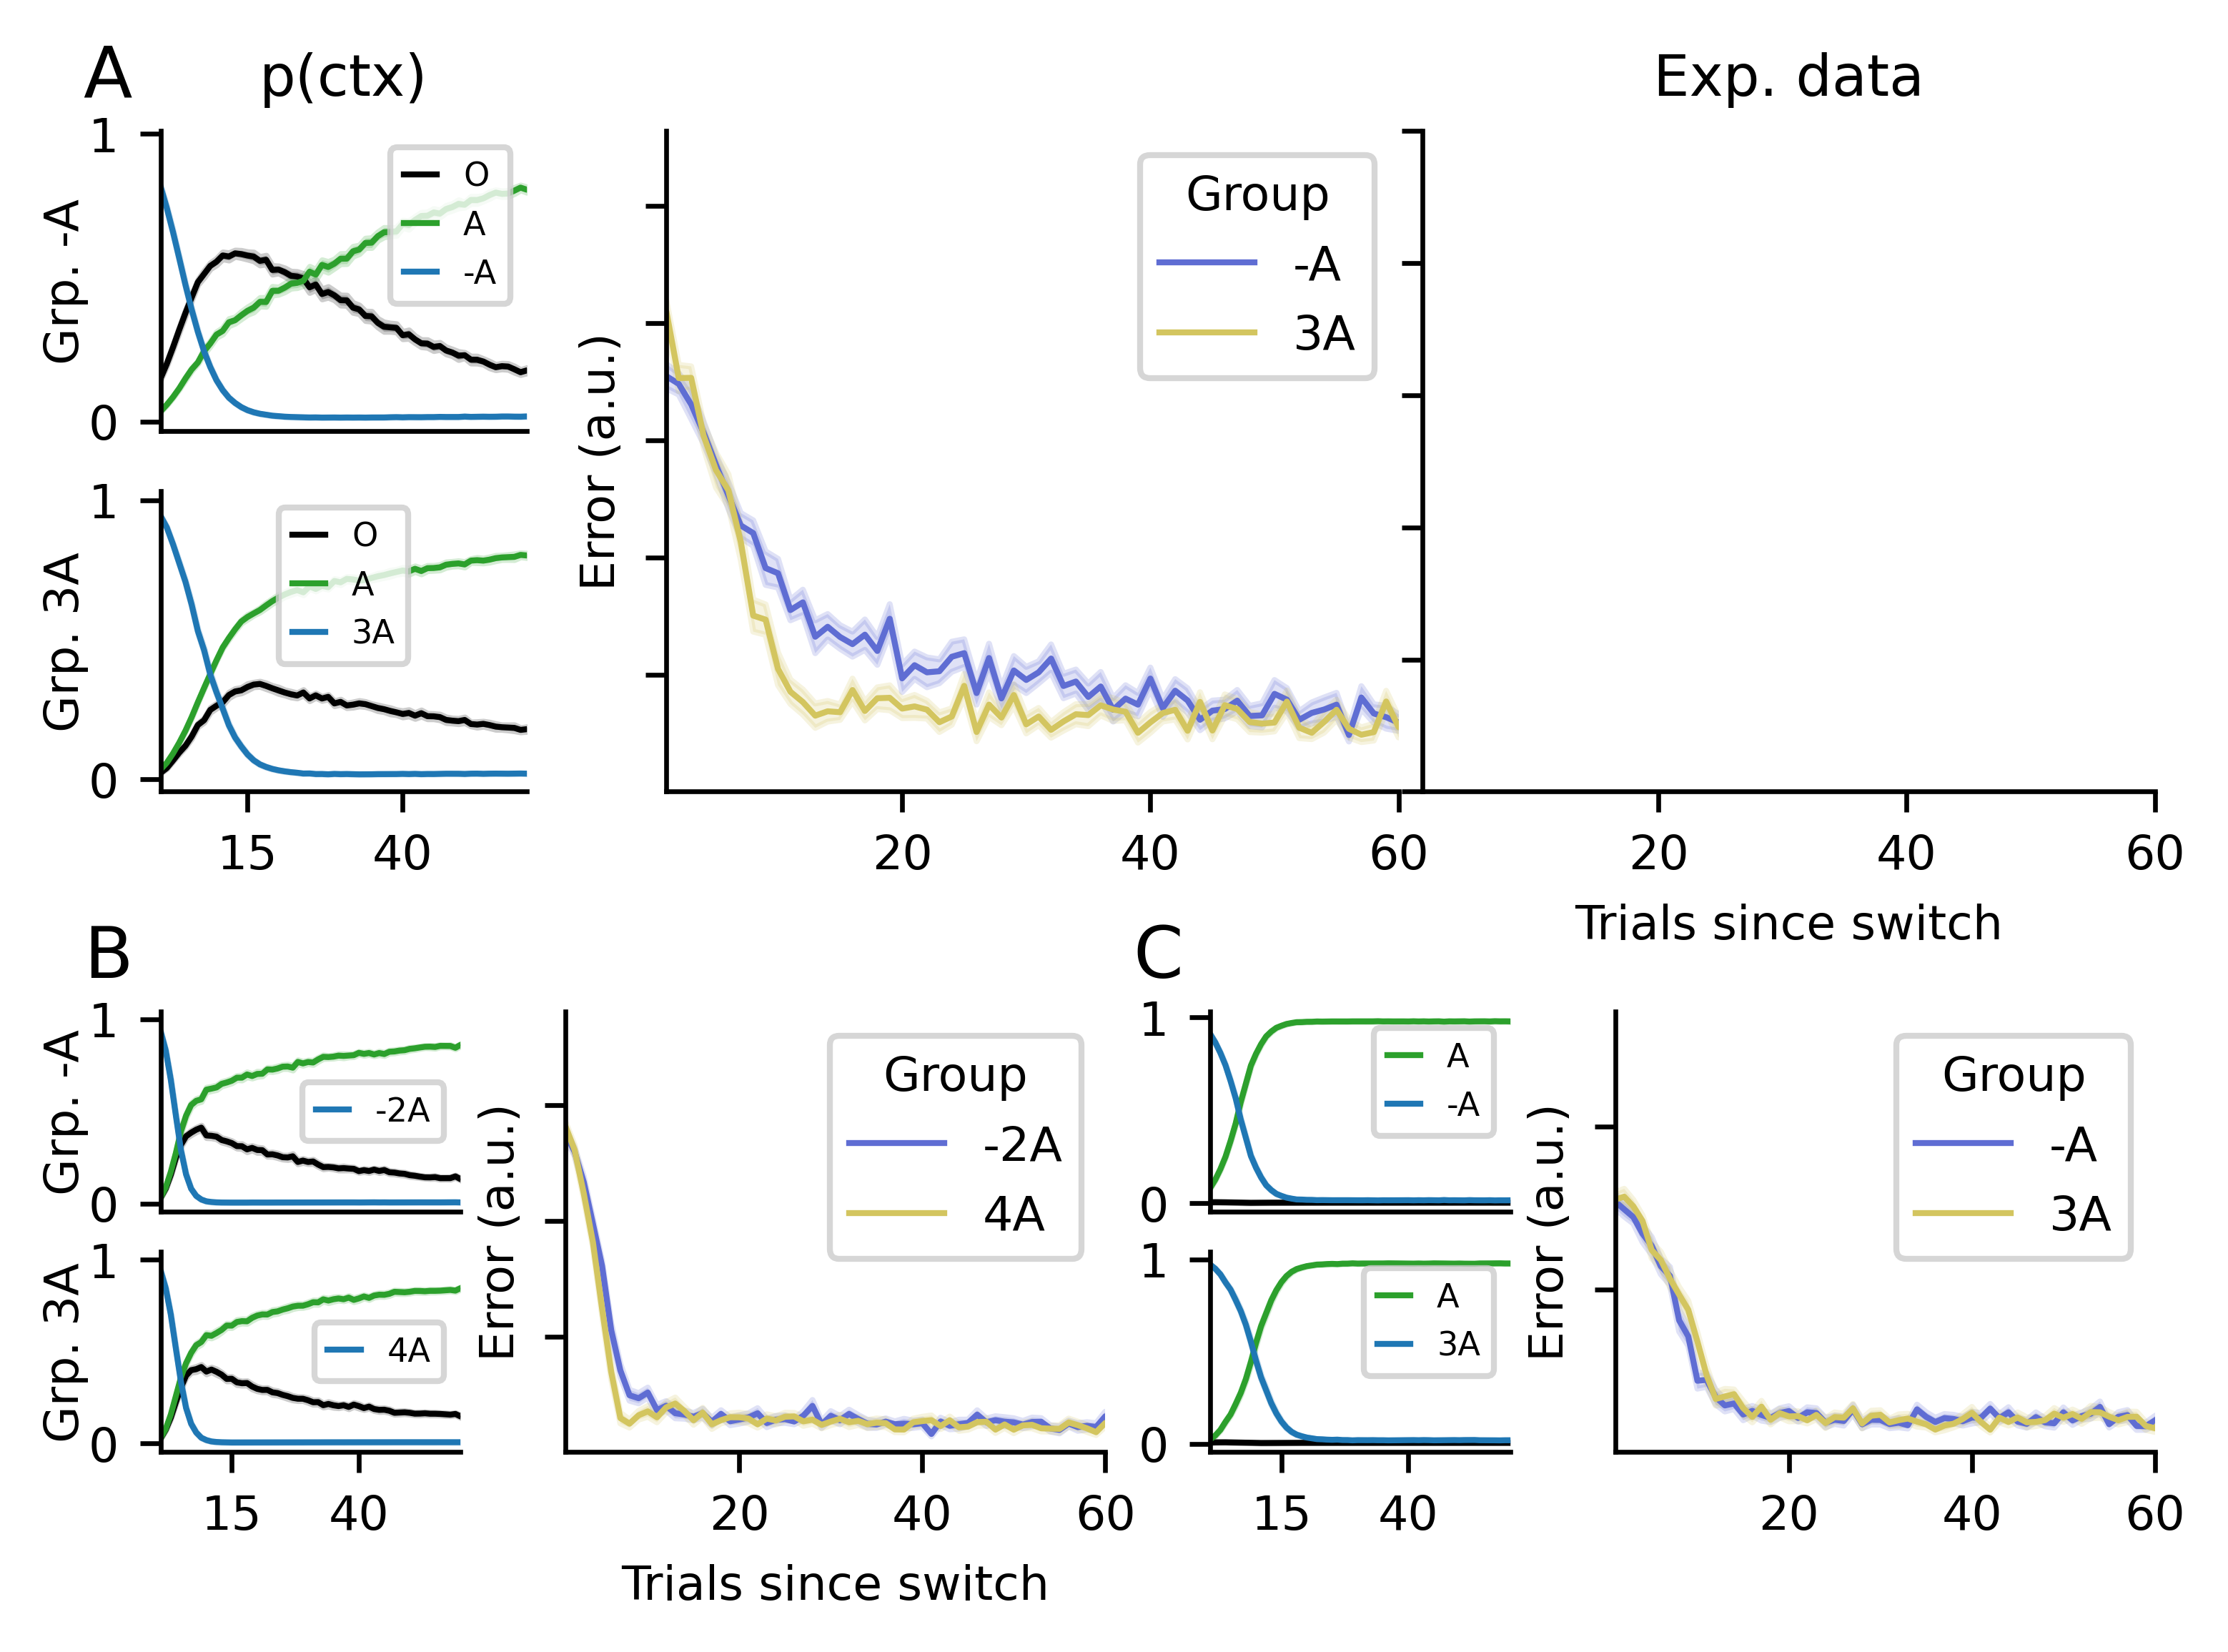
\includegraphics{./figures/figure_3.png}
\caption{Motor error when switching back to a previously learned adaptation. Following the block structure from \cite{Davidson_Scaling_2004}, the first 40 trials of the switch from +8 (yellow) or -8 (blue) to 4 is shown. (A) Simulations from our model, with the task parameters from \cite{Davidson_Scaling_2004}. On the y axis, the error is shown in arbitrary units, related to centimiters through a monotonically increasing transformation with the same origin. (B) Data adapted from \cite{Davidson_Scaling_2004}, showing the error in the same trials as (A).}
\label{fig:davidson-2004}
\end{figure}

Further evidence can be found during error-clamp blocks in several experiments. We discuss these experiments in the following section. Additionally, we discuss experiments similar to that by \cite{Davidson_Scaling_2004} in the Discussion section.


\subsection{Action selection in error-clamp blocks}
During error-clamp blocks at the end of block sequences, participants' behavior can be described as the display of spontaneous recovery (i.e. displaying adaptation consistent with a previously-encountered context) during the early trials of the E block, followed by a slow return to baseline across as many as hundreds of trials \citep{Brennan_Decay_2015}. However, the direction of the spontaneous recovery, its length, the delay before it is observed, the speed of the return to baseline and the final asymptote of the adaptation seem to vary greatly depending on the experiment \citep{Brennan_Decay_2015,Vaswani_Decay_2013,Smith_Interacting_2006,Shmuelof_Overcoming_2012}.

In this section, we show how our model can explain these different parameters of behavior by changing the way contextual cues mislead participants' context inference, which in turn influences action selection.

\cite{Vaswani_Decay_2013} explored in detail human behavior during an error-clamp block in a shooting movement paradigm with a mechanical arm. The authors found that during an E block at the end of each experiment, there was a lag of a few trials (depending on participant) before their motor behavior changed from that of the previous block. After that, the exerted force slowly dropped towards zero throughout tens of trials, but never reaching values around zero. Participants were divided into four groups, each of which going through a different block sequence: (1) A-E, (2) O-A-E, (3) (-A/2)-A-E, and (4) (-A)-E. No pauses were made during the experiment nor were there any contextual cues, so transitions between blocks were not signaled to participants. However, the mechanical arm used in the experiment provided force-feedback to participants.

In \fref{fig:vaswani-2013}A, we show data simulated with our model, following the parameters of the experiment by \cite{Vaswani_Decay_2013}, and in In \fref{fig:vaswani-2013}B we show the experimental data adapted from \cite{Vaswani_Decay_2013}. The displayed adaptation is shown during the E trials for the three experimental groups in the experiment. It can be seen that group 1.3 (i.e. the participants who had learned in the -A/2 context in addition to A) more quickly recognizes that a change in context has occurred and lowers the force applied on the mechanical handle, as can be seen in the experimental data.

\begin{figure}
\centering
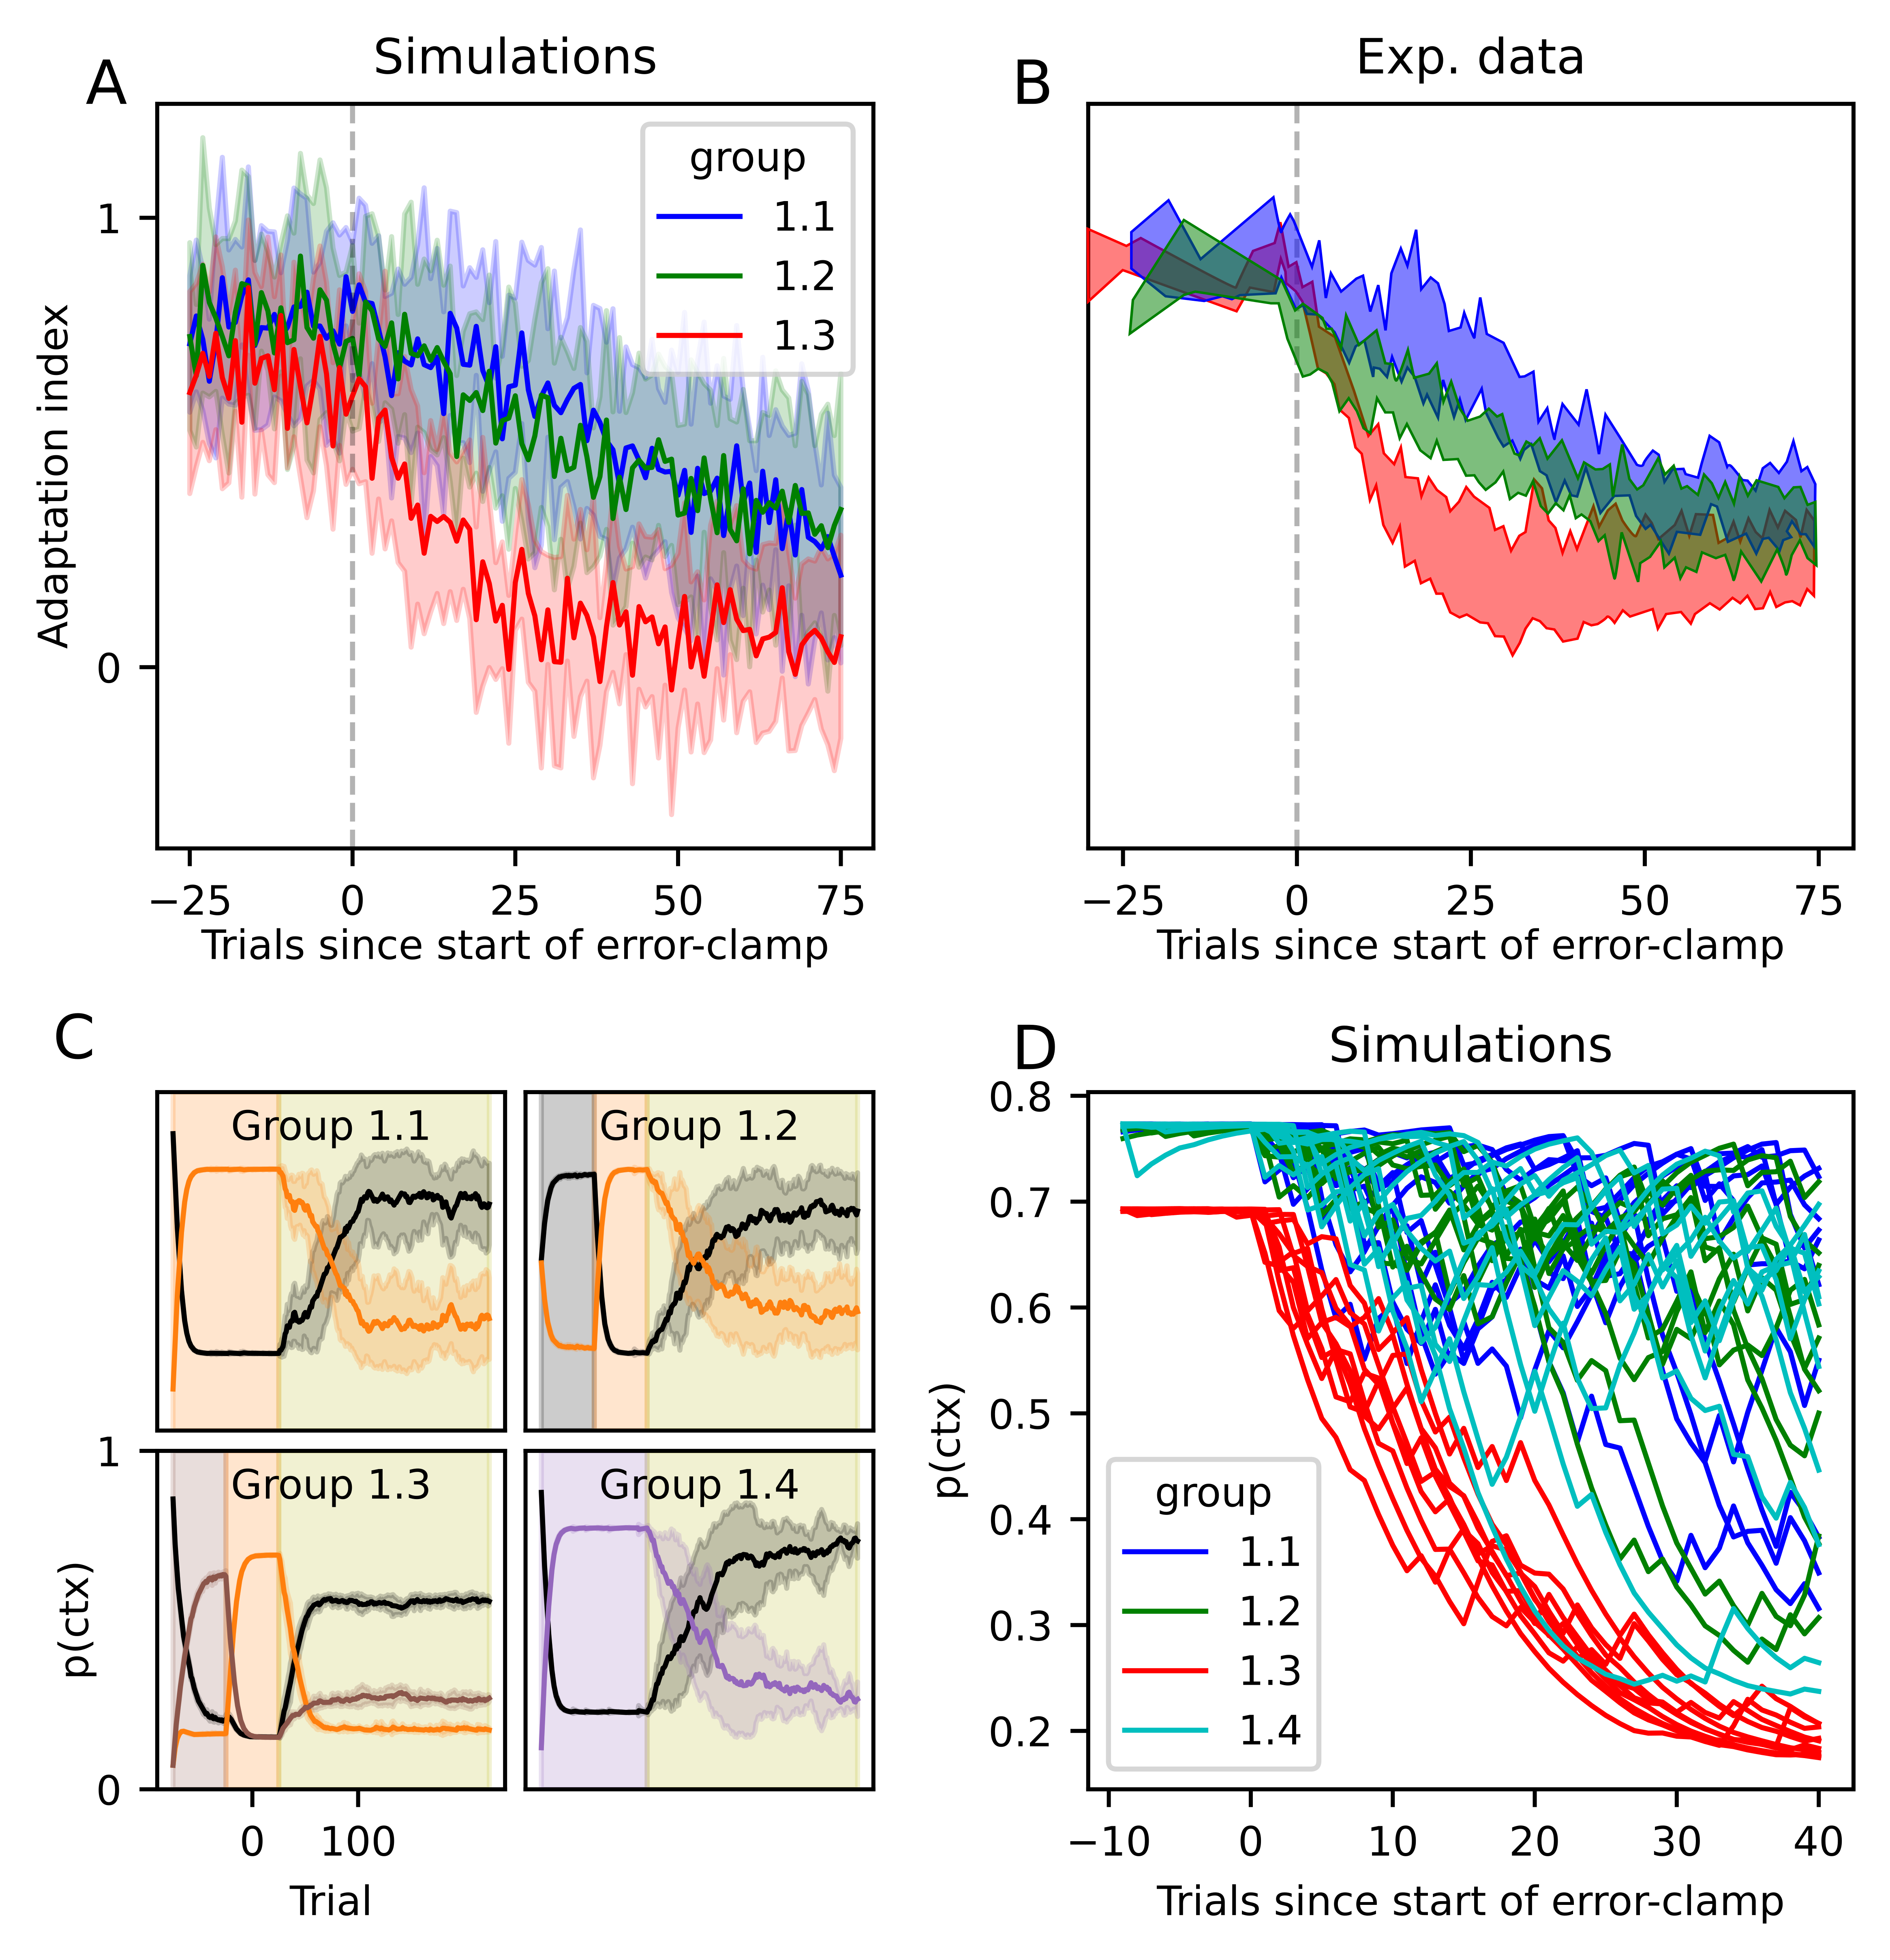
\includegraphics[width=\textwidth]{./figures/figure_4.png}
\caption{Adaptation during error clamp trials. (A) Simulated adaptation during the error-clamp trials for the three groups of participants in \cite{Vaswani_Decay_2013}, using the same colors. The solid line is the average across 10 runs (i.e. 10 simulated participants) and the shaded area represents the standard deviation. The vertical dashed line is the start of the error-clamp trials.(B) Corresponding experimental data adapted from \cite{Vaswani_Decay_2013}. (C) Inference over the current context, where contexts are color coded: black for baseline, orange for the counter-clockwise force, purple for the clockwise force and brown for clockwise force with half strenght. The lines represent the posterior probability of each ocontext at every trial, while the background color represents the real context. An olive-colored background represents error-clamp trials. As in (A), solid lines represent the average across all runs and shaded areas represent the standard deviation. (D) Visualization of the lag before error-clamp trials are detected. Each line represents one run (groups 1.1, 1.2 and 1.3, 10 runs per group).}
\label{fig:vaswani-2013}
\end{figure}

This effect is explained in our model in terms of context inference. In \fref{fig:vaswani-2013}C, the inference over context is shown for each group separately. Context inference works reliably until the error-clamp trials start, which do not correspond to any of the known contexts. This causes the agent to infer the combination of some of the known contexts that best fits the observations. Depending on the contexts previously learned by the agent (which change from group to group), inference during E trials will vary: groups 1.1 and 1.4 have exactly the same behavior, where the previous context (A and -A, respectively) slowly dwindles. These agents will slowly lower the force applied until eventually reaching zero (after hundreds of trials; not shown). In contrast, group 1.3 has learned the additional -A/2 context (represented by brown in \fref{fig:vaswani-2013}C), which has a non-zero posterior probility during E trials, pushing the agent's adaptation force more quickly towards zero. Group 1.2 behaves similarly to 1.1, with the exception that the baseline context, which was recently seen, plays a bigger role during E trials, making the agent reduce its force during E trials slightly more slowly than groups 1.1 and 1.4.


Our model also reproduces the variability in the lag before adaptation starts to drop to zero after the E block starts. In the model, this lag is due to a period in which context inference has not ``caught on'' to the change of context; during this period, behavior remains consistent with that of the previously-observed block, as can be seen in the experimental data as well. To show this, we show in \fref{fig:vaswani-2013}D the drop in the inferred probability of the previous context (A for groups 1.1, 1.2 and 1.3, -A for 1.4) for each simulated run (one line per run, 10 runs per group, all groups). It can be seen that the moment in which the drop starts, as well as the speed of the drops, depends on the run.

\section{Discussion}
We presented a hierarchical model for motor adaptation based on Bayesian inference, which not only learns to adapt its motor outputs by observing errors, but also infers the context in which these arrors were commited and updates the forward model associated with that context.

Similar models have been presented before \cite[e.g.][]{Wolpert_Multiple_1998,Baddeley_System_2003}, which infer the internal models (forward and backward) that best explain the observations and use them to issue motor command. We built on this studies in two important ways: (1) we generalized the inference over the best-fitting internal models to the concept of context inference, which includes all sensory information, in addition to feedback provided by the experimenters or the task; (2) we showed how this seemingly small generalization provides a parsimonious explanation for many experimental phenomena across many experiments in motor adaptation that, up to now, had required multiple \textit{ad hoc} mechanisms.

We selected representative experimental studies that show savings, quick de-adaptation, spontaneous recovery and the effects of sensory cues. Using our model, we showed how each of these effects can be explained by the specifics of context inference, which integrates all the available information (e.g. sensory cues, workspace location, reward and endpoint feedback, etc), in some cases throughout many trials.

It is important to note that the most essential part of the model we presented is the concept of the context and the inclusion of a Bayesian inference scheme over the context, which integrates all the information that is available to the participant during the experiment. The mathematical details of the model are not strictly necessary to reproduce the results. Most notably, we chose to make use of exact Bayesian inference for motor adaptation, with conjugate priors to derive exact update equations. This choice greatly simplifies our simulations and provides very intuitive intepretations for the results. However, we expect the results we presented here to hold using alternative models for motor adaptation, such as Kalman filter-based learners \cite[e.g.][]{Oh_Minimizing_2019,Baddeley_System_2003} and other Bayesian implementations \cite[e.g.][]{Wolpert_Multiple_1998,Kording_Bayesian_2004}. A well established family of models for motor adaptation is linear learners \cite[e.g.][]{Smith_Interacting_2006,Forano_Timescales_2020,Lee_Dual_2009}, however, these models do not incorporate uncertainty in the estimate of the parameters of the internal models, which would limit their implementation in our hierarchical model.

In what follows, we dive deeper into the experimental literature to highlight the importance of contextual information and its effects on observed behavior during motor learning tasks, as shown by our model. In addition, we discuss several predictions that our model makes, which could be verified experimentally in future studies.

\subsection{Extended explanatory power}
Context is often directly observable, either via environmental cues or via feedback observed after actions. In many behavioral experiments, for example, the context of the current block of trials is easily identifiable by the color of a cue light \citep[e.g.][]{Ethier_Spontaneous_2008}, the posture of the hand \citep[e.g.][]{Gandolfo_Motor_1996}, the target of the movement \citep[e.g.][]{Lee_Dual_2009} or by the workspace in which the task is being performed \citep[e.g.][]{Shadmehr_Adaptive_1994}. The context can also be selected by the agent itself. For example, a person can decide the level of care devoted to moving an egg around, which determines the way in which the person would move their hands. In these cases, the context is clearly determined and known to the agent and switches between different adaptations are immediate.

In other cases, however, the context might not be directly observable, and context inference takes the form of an evidence-accumulating process that can take any amount of time to be sure of the context, including infinite. It is in these cases where the effects of context inference are most noticeable. Laboratory experiments with this property are common. While many experiments exist that give probabilistic cues [EGs], or cues that only reveal part of the context [EGs], evidence accumulation is not limited to these explicit cases. Indeed, as we argued in the Results section, many experiments inadvertently include partial contextual information used by participants.

The most direct secondary contextual information comes in the form of reward and endpoint feedback. Participants are told whether they obtained the desired reward at the end of a trial and are shown the end point of their movement. When a participant observes an error that is too large to explain with the expected motor variability, this information can be used to infer that the inferred context might be wrong. This is the case of the experiments by \cite{Oh_Minimizing_2019} shown in \fref{fig:oh-2019}B-C: if the adaptation is high, changes in context produce errors much larger than those of motor variability, and a context switch is easily and immediately identified.; if adaptation is low, the errors produced by context switching are closer in magnitude to motor variability and evidence accumulation is necessary.

The same rationale explains the results from \cite{Davidson_Scaling_2004}: motor learning, which in our model is gated by context inference, is minimal for errors close to 2 and -2 (see their figure 2E). This is because an error of 2 or -2 signals that the participant incorrectly identified the context (as adaptation has a magnitude of 1). It is important to note that they did not calculate a learning of exactly zero in these near-maximal-error trials, which suggests that participants are doing \textit{post hoc} learning: after observing the outcome of their actions, they identify that they had inferred the context incorrectly, and can then adapt the movements for the correct context.

A subtler source of information can be found in long pauses between blocks of adaptation trials. \cite{Ethier_Spontaneous_2008} performed an experiment where the adaptation blocks were divided into sub-blocks of 60 trials each, with a long 30s pause between sub-blocks. The authors observed that at the beginning of each sub-block, participants showed an average dip in their learned adaptation, suggesting that they were partially returning to baseline (O) after each pause. This can be explained by context inference, as a long pause could prompt participants to infer that a switch had occured. Because this was inferred without any information that points at the identity of the new context, prior beliefs take over. This means that participants rely on their belief of the underlying probability of observing any of the known contexts, which is dominated by the previously observed context A, but now includes a component of the baseline O, as it is the most common in their lives.

Error-clamp (E) trials present another insight. During E trials, error is artificially kept at zero. This takes different forms, depending on the type of experiment. If error is kept at zero, one could assume that participants would continue doing what they were doing before, as there is no reason (no observed error) to inferr a change in context. However, this is almost never the case \cite[e.g.][]{Smith_Interacting_2006,Ethier_Spontaneous_2008,Forano_Timescales_2020,Vaswani_Decay_2013,Scheidt_Persistence_2000}. Instead, participants slowly reduce their adaptation, often displaying spontaneous recovery \cite[e.g.][]{Smith_Interacting_2006}, i.e. an initial response in the direction of one of the learned adaptations. Our model provides a principled account of this behavior: while the observed error (i.e. the cursor on the screen) is kept at zero, participants still receive proprioceptive feedback which tells them that something has changed. The natural variability in a participant's behavior will lead her to expect observing errors, which clashes with the observed zero error. This prompts the participant to re-evaluate their inferred context, which can partially activate a previously-learned adaptation, as we showed in \fref{fig:vaswani-2013}. This can be seen in \cite{Criscimagna-Hemminger_Consolidation_2008}, where the authors showed that introducing long periods before the E block begins lowers the initial force that participants exerted on the mechanical arm during the E block; longer periods of time make context inference revert to the prior expectation that a new baseline block begins, because participants are free to move their arm about during the pause \todo{check this}.

In our account, if all information indicating a change in context is removed from the experiment, participants would continue to behave as they were in the previous block. Evidence for this can be seen in experiments 2 and 3 by \cite{Vaswani_Decay_2013}, where they showed random errors to participants during E trials, with a variance matching that of previously observed motor commands. The authors showed that by matching the errors expected by participants, they eliminated the slow tappering off observed in most E blocks. As we showed in \fref{fig:vaswani-2013}D, this effect need not be all or none: in some experimental sessions, participants might fail to notice that a change has occurred due to the stochasticity of their own actions. This would lead to an observed delay before a participant changes her behavior after the E block has started.

[Maybe: talk about generalization in experiments with different workspaces]

\subsection{Model predictions and future work}
The basic principle behind the results we presented is that context inference is a process that develops over time and that carries with it uncertainty. This uncertainty affects learning and behavior, effecting phenomena that are directly observable during behavioral experiments.

In addition to providing a unifying explanation for phenomena such as switching, savings, spontaneous recovery and slow return to baseline, our model makes unique predictions that could be tested in future experiments.

As we already discussed above, the inclusion of reliable sensory contextual cues (e.g. lights whose color uniquely identify a context) makes switching immediate, as in the experiments by \cite{Kim_Neural_2015}. We expect that the same effect would be observed in error-clamp trials. If the E block is learned by participants during training, it might still be difficult for them to identify that an E block has started, which would create delays similar to those in \fref{fig:vaswani-2013}. However, the model predicts that if a visual cue is introduced that identifies the E block, participants would immediately switch to their baseline behavior, no longer displaying spontaneous recovery, lag, nor the slow return to baseline. This immediate switch in the presence of contextual cues would persist even if endpoint feedback is manipulated as \cite{Vaswani_Decay_2013} did.

As we discussed in the Results section, the volatility of the environment (i.e. unpredictable switching between contexts) lowers the measured learning rate. Our model predicts that this effect would be greatly reduced if reliable contextual cues were introduced: if a participant can identify the context of the current trial before any decision or observation has occurred, the learning rate would not be affected by the volatility of the environment. This would manifest in \fref{fig:herzfeld-2014} in the form of no discernible differences between the two groups of participants.

If this prediction is confirmed, our model would additionally suggest that human participants do not revisit the learned adaptation of the last trial when a new observation comes in. To see this, consider the following scenario from the experiments by \cite{Herzfeld_memory_2014}: at trial $t$, the real context was B but the participant inferred context A, issued a motor command consistent with context A and then observed the outcome at $t + 1$. When the outcome is observed, it becomes clear to the participant that the context was B. Does the participant update the internal model of A or of B? According to our model, the participant incorrectly updates A and, upon learning of her mistake at trial $t+1$, does not revert this update. If this were not the case, the volatility of the environment would have no effect, as the context at trial $t$ can almost always be identified at trial $t+1$.

The model also predicts an effect reminescent of multisensory integration: in order to integrate contextual information from conflicting sources (e.g. probabilistic visual cues and noisy endpoint feedback), the weight placed on a source increases with its precision (the inverse of its variance). Such integration would manifest itself in experiments in which observations are noisy, as in the experiments by \cite{Kording_Bayesian_2004}, in which the position of the finger was obscured and instead participants are shown a blurry cursor which was some times shifted from its real position. If the added observation noise gives evidence for a particular context (the real underlying context or another one) and a visual cue gave partial information for another context, the participants' behavior would be more consistent with the most reliable source of contextual information.



\section{Methods}
\subsection{Model description}
\label{subsection:model-description}
We first describe the general principle behind the model, followed, in the next
subsection, by the full mathematical description of each one of its components.

One of the strenghts of this model is that its general principle does not
depend on the specifics of the experiment to which it is applied. However, for
clarity, we will connect the different parts of the model to different
experiments.

Before proceding with the model description, let us introduce nomenclature:
\begin{itemize}
\item $t$: Time at the moment an observation is made, before inference is done.
\item $\theta_t$: Observation. Note that this is assumed to be a noisy
observation of the generalized state (see below) given by $\theta_t = h(z_t)$.
\item $s_t$: Hidden state, e.g. the position of the hand in reaching
experiments. It does not depend on the context.
\item $a_t$: Action taken after observing $\theta_t$ and inferring the context.
\item $c_t$: Context inferred after observing $\theta_t$.
\item $\omega_t$: Contextual information. This term includes, e.g. visual cues,
proprioceptive feedback, performance feedback.
\item $z_t$: Generalized state, $z_t = \{s_t, c_t, \omega_t\}$. Observed noisily
as $\theta_t$.
\end{itemize}

Context inference can work through context-specific (possibly unreliable) sensory cues,
or through the dynamics of the system (e.g. expected outputs of motor
commands), using prediction error as the force behind inference. In this case,
the generative model can is written as follows:
\[
p(z_t, z_{t-1}, a_{t-1}, \theta_t, \theta_{t-1}) = p(\theta_t | z_t)p(z_t|\theta_{t-1}, a_{t-1})
\]
and inferring the current (hidden) generalized state is done with Bayes' theorem:
\[
  q(z_t | \theta_t, \theta_{t-1}, a_{t-1}) \propto p(\theta_t | z_t)p(z_t|\theta_{t-1}, a_{t-1})
\]
  
Additionally, after having inferred the current state, motor adaptation is given by
\[
q(\gamma | z_t, z_{t-1}, a_{t-1}) \propto p(z_t | z_{t-1}, a_{t-1}, \gamma)p(z_{t-1})p(\gamma)
\]

where $\gamma$ are the parameters of the internal model for the dynamics,
i.e. the function $f: (z_t, a_t) \rightarrow z_{t+1}$, which determines the beliefs of
the agent regarding how the system evolves after having taken action $a_t$.

Having inferred the generalized state (including context), a decision is made
sampling from a distribution:
\begin{equation}
p(a_t | z_t, \beta) = \displaystyle\sum_{m \in M}q(C_t)p(a_t | z_t, \beta, m)
\end{equation}
where $M$ is the set of all relevant forward models (see below), and
$p(a_t | ... m)$ is the probability distribution over actions prescribed by the
forward model $m$.

In the following sections, we present a specific mathematical implementation
of the principles outlined above. This is the implementation used throughout the
simulations in the Results section.

\subsubsection{Mathematical implementation}
The generalized state is given by:
\begin{equation}
z_t = \{x, \theta_t, \gamma_t, \omega_t\}
\end{equation}
where $x$ is, e.g. in a reaching task, the current position of the hand in
Cartesian coordinates, where the origin is the starting point. We assume that
motor commands are issued every $\Delta t$ for simplicity. At the beginning of
each time interval, the context is inferred combining the contextual
information and the prediction error of the outcome of the previous motor
command. This yields:
\begin{align}
  q(C_t) &= q(C_t | \omega_t)q(C_t | s_t, s_{t-1}, a_{t-1}) \\ \label{eqn:estimated-context}
  q(C_t | \omega_t) &\propto p(\omega_t | C_t)p(C_t) \\
  q(C_t | x_t, x_{t-1}, a_{t-1}) &\propto p(x_t | C_t, x_{t-1}, a_{t-1})p(x_t)p(x_{t-1})p(C_t)
\end{align}
The terms $p(C_t)$ refer to the prior probability of the context at the
beginning of the trial: at the first trial, this refers to prior beliefs over
which contexts are more common/likely, which we call $p_0(C_t)$. At each
subsequent trial, it incorporates the belief that has so far been accumulated,
given previous trials. Note that certain events, such as the start of a new
block of trials (see main text) can return an agent to a state in which
$p_0(C_t)$ becomes relevant.

We do not directly model hand movements or eye position. Instead, we model
systems in the motor error space: the position $s_t = 0$ represents a trial in
which no motor error occurred. We make use of the fact that in most
experiments, motor adaptation needs to happen in one of two directions
(e.g. clockwise vs. counter-clockwise) to keep the error space
two-dimensional. With this, $s_t > 0$ represents motor error in one direction
(e.g. clockwise) and $s_t < 0$, error in the other direction. We made this
choice because, in this work modeled different experiments with
different state spaces, but with the commonality of (at most)
two-dimensional error spaces. In order to model a specific experiment in its
own physical space (e.g. hand positions in a reaching task), only the dynamical
system would need to be adapted.

We assume that the decision-making agent ha a baseline internal forward models that
map motor commands to outcomes:
\begin{equation}
p(s_{t+1} | s_t, a_t, m) = f_O(s_t, a_t)
\end{equation}
where $a_t$ are motor commands (actions). We further assume that participants
have learned $f_O$ throughout their lives and use it to decide which motor
command to issue under normal circumstances (i.e. no adaptation). When a
perturbation is introduced, to which the participant must adapt, we assume they
learn a new forward model $f_m^{\phi}$, where $\phi$ represents the parameters
of the function that participants must learn. For example, in a saccade task,
$\phi$ represents the new gain. Note that $\phi$ depends on the context and
participants may need to use and update multiple forward adapted models
$f_m^{\phi}$ throughout one experiment.

Given a forward model $f_m$ (or $f_m^\phi$), action selection is done by
building a probability distribution over possible actions $a_t$ based on how
likely they are to produce zero motor error. For example, in saccade
experiments, motor commands are issued based on how likely they are to move the
fovea to the target. These motor commands are issued to counteract intrinsic
sources of error, such as muscle variability and exhaustion, and extrinsic
sources of error, such as the experimental manipulations on saccade gain. Thus,
the expected observed error can be written as:
\begin{equation}
p(\epsilon | a_t) \propto p(\epsilon_{\text{intrinsic}} | a_t) + p(\epsilon_{\text{extrinsic}} | a_t)
\end{equation}
and a motor command can be chosen to maximize the chance of observing zero error:
\begin{equation}
p(a_t) = argmin_{a_t} p(\epsilon | a_t)
\end{equation}

For simplicity, we assume that motor errors are Gaussian, such that:
\begin{equation}
p(\epsilon | a_t) = N(\mu_{\text{extrinsic}}, \sigma_\epsilon)
\end{equation}
where $\sigma_\epsilon$ incorporates both intrinsic and extrinsic sources of
error and is a free parameter of the model. The mean of the error is assumed to
have no intrinsic component, as motor commands, in the absence of external
errors, should produce an error centered at zero [CITATION MISSING].

With this, a forward model will produce a motor command with outcomes centered
at $-\mu_{\text{extrinsic}}$, which counteracts the externally-induced errors.

To complete the action-selection picture, we return to context inference. As
discussed above, action selection is made via a weighted sum of the different
forward models:
\begin{equation}
p(a_t | ...) \propto \displaystyle \sum_{m \in M} q(C_i)p(a_t | m)
\end{equation}
From this distribution, an action is sampled at each trial.

To update the agent's estimates on the parameters of the forward models, we
make use of Bayes' theorem with conjugate priors. This approach has the
advantage of not only greatly simplifying computational calculations, but also
presenting update equations with great intuitive appeal.

In the following equations, we drop the dependence on the context and
observations for notational simplicity:
\begin{equation}
q(\phi | s_{1:t}) \propto p(s_{1:t} | \phi)p(\phi)
\end{equation}
where $s_{1:t}$ are the observed states up until time $t$. The likelihood will
be a Gaussian:
\begin{align}
  p(s_t | \theta) &= N(\mu_x, \sigma_x)  \\
  \mu_x &= \theta_{t-1} + x \\
  \sigma_x &= \xi_0 1
\end{align}
This likelihood is the probability of observing $x$ given the previous estimate
of the parameters of the force field $\phi_{t-1}$, and given the dynamics of
the system (see below).

To update $\phi$, we assumed that for each context, the agent's belief over
the magnitude of the adaptation is given by a normal distribution:
\begin{equation}
p(\phi) = N(\mu_\phi, \sigma_\phi) \label{eqn:data-dist}
\end{equation}
where $\mu_\phi$ and $\sigma_\phi$ are parameters to be estimated at each
trial. Before the experiment begins, the agent will have a prior distribution
over these parameters. A standard Bayesian approach is to choose NormalGamma
priors:
\begin{equation}
p(\mu_\phi, \sigma_\phi) = NG(\mu_0, \nu_0, \alpha_0, \beta_0)
\end{equation}
where $\mu_{\phi}^0, \nu_{\phi}^0, \alpha_{\phi}^0$ and $\beta_{\phi}^0$ are free hyperparameters of the
model.

The update equations for the magnitud parameters are given by:
\begin{equation}
q(\mu_f, \sigma_f | x_t, x_{t-1}, a_{t-1}) \propto p(x_t |
x_{t-1}, a_{t-1}, C_t)p(\mu_f, \sigma_f) \label{eqn:context-from-x}
\end{equation}
where $p(x_t | x_{t-1}, a_{t-1}, C_t)$ is a Gaussian distribution centered
around $\mu_a$ with standard deviation $\sigma_a$, which is a free parameter of
the model. It is assumed that the standard deviation over outcomes ($\sigma_a$)
is related to that of the parameter $\mu_f$ as follows:
\begin{equation}
\sigma_f = \sigma_a / \nu_f
\end{equation}
which makes $\nu_f$ a parameter to estimate. Each one of the forward models can
be updated at every trial, depending on context inference (see main text). The
updated parameters for any one forward model $i$ are given by:
\begin{align}
  \mu_\phi^{(t)} &= \frac{\nu_\phi^{(t-1)} \mu_\phi^{(t-1)} + q(C_i)s_t}{\nu_\phi^{(t-1)} + q(C_i)} \\
  \nu_\phi^{(t)} &= \nu_\phi^{(t-1)} + q(C_i) \\
  \alpha_\phi^{(t)} &= \alpha_\phi^{(t-1)} + q(C_i) / 2 \\
  \beta_\phi^{(t)} &= \beta_\phi^{(t-1)} + \frac{q(C_i)\nu_\phi^{(t-1)}}{\nu_\phi^{(t-1)} +
                  q(C_i)}\frac{\left(s_t - \mu_\phi^{(t-1)}\right)^2}{2}
\end{align}
where $q(C_i)$ is the posterior probability of context $C_i$ from
\eref{eqn:estimated-context}. Note that when $q(C_i) = 0$, the model $i$ is not
updated.

\subsubsection{Interpreting the hyperparameters}
Naturally, $\mu$ affects the initial estimate of the adaptation, in the same
units as the necessary adaptation. $\nu$ encodes how stable this hyperprior is:
higher values (e.g. 10000) all but guarantee that the hypermean will not move
in the face of evidence; In principle, enough evidence should still move it,
but that won't happen during an experiment. Smaller values (e.g. 1 / force\_sd,
as is the default on the code) make the hypermean (and thus the mean) follow
evidence more freely. Note that as more observations are accumulated, $\nu$
becames bigger and bigger, solidifying the value of the hypermean.

The hyperparameters $\alpha$ and $\beta$ have a more complex effect. Note that the
mean of a Gamma distribution is $1 / (\alpha \nu)$; this mean is being used
as the standard deviation of a Gaussian by the rest of the agent (cheating),
which makes it an important measure of uncertainty. While setting the default
hyperparameters, the values used are $\alpha = 0.5 / \sigma_0$ and
$\beta = 0.5$, where $\sigma_0$ is the \textit{a priori} estimate of the
standard deviation of the force exerted by the environment (force\_sds in the
code), which controls the initial learning rate. This makes the initial
standard deviation equal $\sigma_0$, which makes it consistent with the
fixed-force model in its interface. The 0.5 values ensure that uncertainty is
large at the beginning and during the experiment is greatly reduced, but never
to a point where it's ``visually'' too small. Changing this 0.5 would make the
standard deviation change more quickly, making the model more or less precise
in its predictions, independently of the volatility of the mean of the
adaptation (via the hypermean).

The baseline model defaults to different values that make it a lot more
stable. The hyperstd of the mean is set to 10,000, which makes the mean
entirely stable during the duration of the experiment. The values of $\alpha$
and $\beta$ are fixed regardless of $\sigma_0$ such that the standard deviation
is 0.001 (compare that to the size of the adaptations, around 0.0125), and the
hyperparameters of the standard deviation are stable during the experiment.


\bibliography{../../MyLibrary}


\end{document}
